\section{Exponential Functions}
\label{sec:exp}

\subsection{Laws of Exponents}
\label{ssec:laws-exp}

The Laws of Exponents let you rewrite algebraic expressions that involve exponents. The last three listed here are really definitions rather than rules.

\begin{theorem}[Laws of Exponents\index{Laws of Exponents}]
All variables here represent real numbers and all variables in denominators are nonzero.
\begin{enumerate}
    \item $x^a\cdot x^b=x^{a+b}$
		\item $\dfrac{x^a}{x^b}=x^{a-b}$
		\item $\left(x^a\right)^b=x^{ab}$
		\item $(xy)^a=x^a y^a$
		\item $\left(\dfrac{x}{y}\right)^b=\dfrac{x^b}{y^b}$
		\item $x^0=1$, provided $x\neq 0$, although in some contexts, $0^0 = 1$.
		\item $x^{-n}=\dfrac{1}{x^n}$, provided $x\neq 0$.
		\item $x^{1/n}=\sqrt[n]{x}$, provided $x\neq 0$.
\end{enumerate}
\end{theorem}

\begin{example}
Simplify $\left(2x^2\right)^3(4x)$.

\solution We'll begin by simplifying the $\left(2x^2\right)^3$ portion. Using Property 4, we can write
\begin{align*}
\left(2x^2\right)^3 &= 2^3\left(x^2\right)^3(4x)& &\mbox{Use Property 4.}\\
  &= 8x^6(4x)&                  &\mbox{Evaluate $2^3=8$, and use Property 3.}	\\
  &= 32x^7&                     &\mbox{Multiply the constants, and use Property 1, recalling $x=x^1$.}
\end{align*}
\end{example}

Being able to work with negative and fractional exponents will be very important later in this course.

\begin{example}
Rewrite \(\dfrac{5}{x^3}\) using negative exponents.

\solution Since \(x^{-n}=\dfrac{1}{x^n}\), then \(x^{-3}=\dfrac{1}{x^3}\) and thus
\[\dfrac{5}{x^3}=5x^{-3}.\]
\end{example}

\begin{example}
Simplify \(\left(\dfrac{x^{-2}}{y^{-3}}\right)^2\) as much as possible and write your answer using only positive exponents.

\solution
\begin{align*}
		\left(\dfrac{x^{-2}}{y^{-3}}\right)^2 &=  \dfrac{\left(x^{-2}\right)^2}{\left(y^{-3}\right)^2}\\
		 &=  \dfrac{x^{-4}}{y^{-6}}\\
		 &=  \dfrac{y^6}{x^4}
	\end{align*}
\end{example}

\begin{example}
Rewrite \( \left(\sqrt{p^5}\right)^{-1/3} \) using exponents.

\solution A square root is a radical with index of two. In other words, \(\sqrt{x}=\sqrt[2]{x}\). Using the exponent rule above, \(\sqrt{x}=\sqrt[2]{x}=x^{1/2}\). Rewriting the square roots using the fractional exponent, \[4\sqrt{x}-\dfrac{3}{\sqrt{x}}=4x^{1/2}-\dfrac{3}{x^{1/2}}.\]

Now we can use the negative exponent rule to rewrite the second term in the expression:
\[4x^{1/2}-\dfrac{3}{x^{1/2}}=4x^{1/2}-3x^{-1/2}.\]
\end{example}

\begin{example}
Rewrite \( \left(\sqrt{p^5}\right)^{-1/3} \) using only positive exponents.

\solution
  \begin{align*}
		\left(\sqrt{p^5}\right)^{-1/3} &=  \left(\left(p^5\right)^{1/2}\right)^{-1/3}\\
		 &=  p^{-5/6}\\
		 &=  \frac{1}{ p^{5/6}}
	\end{align*}
\end{example}

\begin{example}
Rewrite \( x^{-4/3} \) as a radical.

\solution
\begin{align*}
		x^{-4/3} &=  \frac{1}{x^{4/3}} \\
		 &=  \frac{1}{\left(x^{1/3}\right)^4} \quad \text{(since \(\frac{4}{3}=4\cdot\frac{1}{3}\))}\\
		 &=  \frac{1}{\left(\sqrt[3]{x}\right)^4} \quad \text{(using the radical equivalence)}
	\end{align*}
\end{example}

\subsection{Exponential Models}
\label{ssec:models-exp}

Consider these two companies:
\begin{itemize}
  \item Company A has 100 stores, and expands by opening 50 new stores a year
  \item Company B has 100 stores, and expands by increasing the number of stores by 50\% of their total each year.
\end{itemize}
Company A is exhibiting linear growth. In linear growth, we have a constant rate of change -- a constant number that the output increased for each increase in input. For company A, the number of new stores per year is the same each year.

Company B is different -- we have a percent rate of change rather than a constant number of stores/year as our rate of change. To see the significance of this difference compare a 50\% increase when there are 100 stores to a 50\% increase when there are 1000 stores:
\begin{itemize}
  \item 100 stores, a 50\% increase is 50 stores in that year.
  \item 1000 stores, a 50\% increase is 500 stores in that year.
\end{itemize}
Calculating the number of stores after several years, we can clearly see the difference in results.

\begin{table}[!ht]
  \centering
  \begin{tabular}{rrr}
    \toprule
    Years	& Company A	& Company B	\\
    \midrule
    2	 & 200 & 	225	\\
    4	& 300	& 506	\\
    6	& 400	& 1139	\\
    8	& 500 &	2563	\\
    10&	600 & 	5767\\
    \bottomrule
  \end{tabular}
\end{table}

\begin{figure}[!ht]
\centering
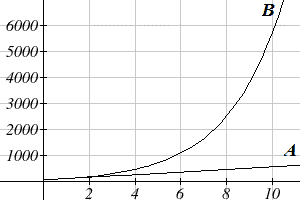
\includegraphics[width=0.5\textwidth]{img/chap1/sec1-6/image072.png}
\caption{Graphs of data from A and B, with B fit to a curve.}
\end{figure}

This percent growth can be modeled with an {\bf exponential function}\index{Function!exponential}.

\begin{definition}[Exponential Function]
An {\bf exponential growth}\index{Exponential growth} or {\bf decay}\index{Exponential decay} function is a function that grows or shrinks at a constant percent growth rate. The equation can be written in the form
$$f(x) = a\cdot(1+r)^x$$
or
$$f(x)=a\cdot b^x \enspace ,$$
where
\begin{itemize}
  \item[$a$] is the {\bf initial or starting value}\index{Initial value}\index{Starting value} of the function,
  \item[$r$] is the {\bf percent growth or decay rate}\index{Rate!decay}\index{Rate!growth}, written as a decimal,
  \item[$b$] is the {\bf growth factor}\index{Growth factor} or {\bf growth multiplier}\index{Growth multiplier}: $b=1+r$.
\end{itemize}
Since powers of negative numbers behave strangely, we must have $b>0$.
\end{definition}

\begin{example}
India's population was 1.14 billion in the year 2008 and is growing by about 1.34\% each year. Write an exponential function for India's population, and use it to predict the population in 2020.

\solution Using 2008 as our starting time ($t=0$), our initial population will be 1.14 billion. Since the percent growth rate was 1.34\%, our value for $r$ is 0.0134.

Using the basic formula for exponential growth $f(x)=a(1+r)^xx$, we can write the formula,
$$f(t)=1.14(1+0.0134)^t$$
To estimate the population in 2020, we evaluate the function at $t=12$, since 2020 is 12 years after 2008:
$$f(t)=1.14(1+0.0134)^{12}\approx1.337 \mbox{ billion people in 2020.}$$
\end{example}

\begin{example}
A certificate of deposit (CD) is a type of savings account offered by banks, typically offering a higher interest rate in return for a fixed length of time you will leave your money invested. If a bank offers a 24 month CD with an annual interest rate of 1.2\% compounded monthly, how much will a \$1000 investment grow to over those 24 months? What is the equivalent annual percentage yield (APY)?

\solution First, we must notice that the interest rate is an annual rate, but is compounded monthly, meaning interest is calculated and added to the account monthly. To find the monthly interest rate, we divide the annual rate of 1.2\% by 12 since there are 12 months in a year: $\frac{1.2\%}{12} = 0.1\%$. Each month we will earn 0.1\% interest. From this, we can set up an exponential function, with our initial amount of \$1000 and a growth rate of $r=0.001$, and our input $m$ measured in months:
$$f(m)=1000\left(1+\frac{0.012}{12}\right)^m=1000(1.001)^m \enspace .$$
After 24 months, the account will have grown to $f(24)=1000(1.001)^{24}\approx\$1024.28.$

The annual percentage yield (APY) is the interest rate that is equivalent to 1.2\% compounded quarterly if we were to compound annually instead. So we will calculate how much our investment grows in one year (expressed as a percentage of the original amount), which means using $m=12$ months:
$$f(12)=1000(1.001)^{12}\approx\$1012.07 \enspace ,$$
so we have
$$\frac{\mbox{Final value}}{\mbox{Initial value}} = \frac{\$1012.07}{\$1000}=1.01207$$
or $101.207\%$ of what we started with, which is a 1.207\% gain. Thus our APY is 1.207\%. This answer seems reasonable since when compounding quarterly we earn interest on interest from the previous quarters, so to compensate for the fact that we are not compounding as often we need a slightly higher rate to earn an equal amount.
\end{example}

\begin{example}
Bismuth-210 is an isotope that radioactively decays by about 13\% each day, meaning 13\% of the remaining Bismuth-210 transforms into another atom (Polonium-210 in this case) each day. If you begin with 100 mg of Bismuth-210, how much remains after one week?

\solution With radioactive decay, instead of the quantity increasing at a percent rate, the quantity is decreasing at a percent rate. Our initial quantity is $a=100$ mg, and our growth rate will be negative 13\%, since we are decreasing: $r=-0.13$. This gives the equation
$$Q(d)=100(1-0.13)^d=100(0.87)^d \enspace .$$
This can also be explained by recognizing that if 13\% decays, then 87 \% remains.

After one week, 7 days, the quantity remaining would be $Q(7)=100(0.87)^7=37.73$ mg of Bismuth-210.
\end{example}

\begin{example}
$T(q)$ represents the total number of Android smart phone contracts, in thousands, held by a certain Verizon store region measured quarterly since January 1, 2010. Interpret all of the parts of the equation $T(2)=86(1.64)^2=231.3056$ .

\solution Interpreting this from the basic exponential form, we know that 86 is our initial value. This means that on Jan. 1, 2010 this region had 86,000 Android smart phone contracts. Since $b=1+r=1.64$, we know that every quarter the number of smart phone contracts grows by 64\%. $T(2)=231.3056$ means that in the second quarter (or at the end of the second quarter) there were approximately 231,305 Android smart phone contracts.
\end{example}

When working with exponentials, there is a special constant we must talk about. It arises when we talk about things growing continuously, such as continuous compounding, or natural phenomena like radioactive decay that happen continuously.

\begin{definition}[Euler's Number: $e$]
$$e\approx2.718282$$
\end{definition}
Because $e$ is often used as the base of an exponential, most scientific and graphing calculators have a button that can calculate powers of $e$, usually labeled $e^x$. Some computer software instead defines a function $\exp(x)$, where $\exp(x) = e^x$. Since calculus studies continuous change, we will almost always use the $e$-based form of exponential equations in this course.

\begin{definition}[Continuous Growth Formula]
{\bf Continuous growth}\index{Continuous growth} can be calculated using the formula
$$f(x)=a\cdot e^{rx} \enspace ,$$
where
\begin{itemize}
    \item[$a$] is the {\bf starting amount}\index{Initial value}\index{Starting value} or {\bf initial quantity},
    \item[$r$] is the {\bf continuous growth rate}\index{Growth rate}.
\end{itemize}
\end{definition}

\begin{example}
Radon-222 decays at a continuous rate of 17.3\% per day. How much will 100mg of Radon-222 decay to in 3 days?

\solution Since we are given a continuous decay rate, we use the continuous growth formula. Since the substance is decaying, we know the growth rate will be negative: $r=-0.173$, $f(3)=100e^{-0.173\cdot 3}\approx 59.512$ mg of Radon-222 will remain.
\end{example}

\subsection{Graphs of Exponential Functions}
\label{ssec:graphs-exp}

\begin{theorem}[Graphical Features of Exponential Functions]
In the graph of the function $f(x) = a\cdot b^x$, we have the following.

\begin{itemize}
  \item $a$ is the {\bf vertical intercept} of the graph.
  \item $b$ determines the {\bf rate} at which the graph grows:
  \begin{itemize}
      \item the function will {\bf increase} if $b>1$,
      \item the function will {\bf decrease} if $0<b<1$.
  \end{itemize}
  \item The graph will have a {\bf horizontal asymptote} at $y=0$.
  \item The graph will be:
  \begin{itemize}
    \item {\bf concave up} if $a>0$
    \item {\bf concave down} if $a<0$.
  \end{itemize}
  \item The {\bf domain} of the function is all real numbers, $\R$.
  \item The {\bf range} of the function is $(0,\infty)$ if $a>0$, and $(-\infty,0)$ if $a<0$.
\end{itemize}
\end{theorem}

When sketching the graph of an exponential function, it can be helpful to remember that the graph will pass through the points $(0,a)$ and $(1, ab)$.

\begin{theorem}
The value $b$ will determine the function's long run behavior. The notation $x\to\infty$ means ``as the value of $x$ grows (without bound) to infinity ($\infty$)," or, more briefly, ``as $x$ goes to $\infty$."
\begin{itemize}
  \item If $b>1$:
  \begin{itemize}
    \item As $x\rightarrow\infty$, $f(x)\rightarrow\infty$.
    \item As $x\rightarrow-\infty$, $f(x)\rightarrow 0$.
  \end{itemize}
  \item If $0<b<1$:
  \begin{itemize}
    \item As $x\rightarrow\infty$, $f(x)\rightarrow 0$.
    \item As $x\rightarrow-\infty$, $f(x)\rightarrow\infty$.
  \end{itemize}
\end{itemize}
\end{theorem}

\begin{example}
Sketch a graph of $f(x) = 4\cdot \left(\frac{1}{3}\right)^x$.

\solution This graph will have a vertical intercept at the point $(0,4)$, and passes through the point $\left(1,\frac{4}{3}\right)$. Since $b<1$, the graph will be decreasing towards zero. Since $a>0$, the graph will be concave up.

\begin{figure}[!ht]
\centering
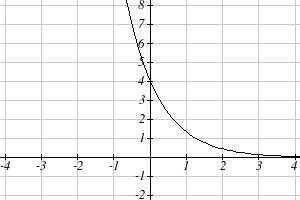
\includegraphics[width=0.5\textwidth]{img/chap1/sec1-6/image073.png}
\caption{}
\end{figure}
We can also see from the graph the long run behavior: as $x\rightarrow\infty$, $f(x)\rightarrow 0$, and as $x\rightarrow-\infty$, $f(x)\rightarrow\infty$.
\end{example}

To get a better feeling for the effect of the coefficients $a$ and $b$ on the graph, examine the sets of graphs below. The first set shows various graphs, where $a$ remains the same and we only change the value for $b$. Notice that the closer the value of $b$ is to 1, the less steep the graph will be.

\begin{figure}[!ht]
\centering
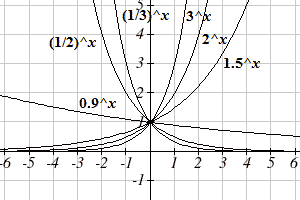
\includegraphics[width=0.5\textwidth]{img/chap1/sec1-6/image074.png}
\caption{Changing the value of $b$.}
\end{figure}

In the next set of graphs, $a$ is altered and our value for $b$ remains the same.

\begin{figure}[!ht]
\centering
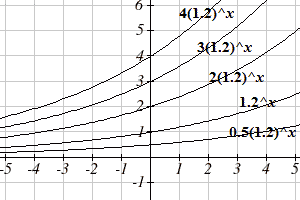
\includegraphics[width=0.5\textwidth]{img/chap1/sec1-6/image075.png}
\caption{Changing the value of $a$.}
\end{figure}

Notice that changing the value for $a$ changes the vertical intercept. Since $a$ is multiplying the $b^x$ term, $a$ acts as a vertical stretch factor, not as a shift. Notice also that the long run behavior for all of these functions is the same because the growth factor did not change and none of these $a$ values introduced a vertical flip.

%[Try it for yourself using this applet:]

\begin{example}
Match each equation with its graph.
\begin{itemize}
  \item[] $f(x)=2(1.3)^x$
  \item[] $g(x)=2(1.8)^x$
  \item[] $h(x)=4(1.3)^x$
  \item[] $k(x)=4(0.7)^x$
\end{itemize}
\begin{figure}[!ht]
\centering
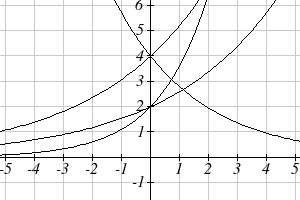
\includegraphics[width=0.5\textwidth]{img/chap1/sec1-6/image076.png}
\caption{}
\end{figure}
\solution The graph of $k(x)$ is the easiest to identify, since it is the only equation with a growth factor less than $1$, which will produce a decreasing graph. The graph of $h(x)$ can be identified as the only growing exponential function with a vertical intercept at the point $(0,4)$. The graphs of $f(x)$ and $g(x)$ both have a vertical intercept at $(0,2)$, but since $g(x)$ has a larger growth factor, we can identify it as the graph that is increasing faster.

\begin{figure}[!ht]
\centering
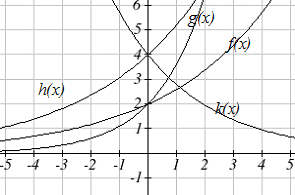
\includegraphics[width=0.5\textwidth]{img/chap1/sec1-6/image077.png}
\caption{}
\end{figure}

\end{example}

\subsection{Exercises}
\label{ssec:1-6-exercises}
\begin{enumerate}
\item[] Simplify each expression.
\item $x^3x^5$
\item $x^4x^2$
\item $(x^3)^4$
\item $(x^7)^2$
\item $(2x^2)^3x^4$
\item $(5x^4)^2 x^5$
\item $\frac{(3x^2)^2}{6x^3}$
\item $\frac{5x(4x)^2}{2x^2}$

\item[] Simplify, and rewrite without negative exponents.
\item $4x^{-3}$
\item $2x^{-5}$
\item $x^{-4}x^2$
\item $x^{-2}x$
\item $\frac{5x^{-3}}{2x^{-6}}$
\item $\frac{2x^{-4}}{6x^{-2}}$

\item[] Rewrite using negative or fractional exponents.
\item $\frac{4}{x^{5}}$
\item $\frac{4}{x^3}$
\item $3\sqrt{x}$
\item $\sqrt[4]{x}$
\item $\frac{4}{\sqrt[3]{x}}$
\item $\frac{1}{5\sqrt{x}}$

\item[] Rewrite as a radical.
\item $4x^{-1/2}$
\item $5x^{-1/3}$
\item $2x^{1/3}$
\item $5x^{3/2}$


  \item A population numbers 11,000 organisms initially and grows by 8.5\% each year.  Write an exponential model for the population.

  \item A population is currently 6,000 and has been increasing by 1.2\% each day.  Write an exponential model for the population.

\item A vehicle purchased for \$32,500 depreciates at a constant rate of 5\% each year. Determine the approximate value of the vehicle 12 years after purchase.

\item A business purchases \$125,000 of office furniture which depreciates at a constant rate of 12\% each year.  Find the residual value of the furniture 6 years after purchase.

\item If \$4,000 is invested in a bank account at an interest rate of 7 per cent per year, find the amount in the bank after 9 years if interest is compounded annually, quarterly, monthly, and continuously.

\item If \$6,000 is invested in a bank account at an interest rate of 9 per cent per year, find the amount in the bank after 5 years if interest is compounded annually, quarterly, monthly, and continuously.
Match each function with one of the graphs below.

\item $f(x) = 2(0.69)^x$
\item $f(x) = 2(1.28)^x$
\item $f(x) = 2(0.81)^x$
\item $f(x) = 4(1.28)^x$
\item $f(x) = 2(1.59)^x$
\item $f(x) = 4(0.69)^x$

If all the graphs to the right have equations with form $f(t) = a\cdot e^{kt}$,
\item Which graph has the largest value for $k$?
\item  Which graph has the smallest value for $k$?
\item  Which graph has the largest value for $a$?
\item  Which graph has the smallest value for $a$?
\end{enumerate}
